\evenchapter{Création du portail cartographique}

\textit{Ce chapitre présente le travail de mise en ligne du portail cartographique sur la plateforme ArcGIS Online de la Direction des Affaires Foncières}

\section{Fond de plan multi-échelle}

\textit{Jusqu'à présent, chaque niveau d'échelle était représenté par une carte distincte. L'export sur ArcGIS Online a nécessité le regroupement des projets et la création d'un projet nommé "export\_web" entièrement dédié à l'export web.}





\subsection{ Paramètres de l'export}

\textit{ArcGIS propose différentes façons d’exporter un projet, en carte web ou en couche web. }

La carte web a vocation première de basculer un projet d’ArcGIS PRO vers le web avec la possibilité de faire évoluer le projet sur le web sur les aspects de symbologie et d’étiquetage.Elle nécessite le choix d’un fond de carte pour être diffusée.  L’export de couches web, quant à lui,  est dédié au partage de la donnée sur ArcGIS Online. La donnée peut ensuite être reprise au sein de cartes web afin de la diffuser et/ou de la structurer. Le géotraitement qui réalise cet export permet de définir le format de partage de la donnée en couche d'entités, en tuile raster ou bien en tuiles vectorielles. \\

L’export en couches web a été choisi pour les raisons suivantes : 

\begin{itemize}
\item la symbologie a été élaborée au sein d’ArcGIS PRO et il n’est pas souhaitable de reprendre la symbologie sur le web ; 
\item  La carte web nécessite le choix d’un fond de carte. Or, le but du projet étant de réaliser un fond de carte, cela aurait été problématique ; \\
\end{itemize}

    Pour des raisons de performances, le choix technique du format d’export s'est été porté sur les tuiles vectorielles. L’export en carte web ne permet pas ce type de format de stockage des données. Les différents formats seront détaillés plus bas et le choix des formats d’export justifié.  

\begin{table}[]
\small
\begin{tabular}{|cc|c|l|l|}
\hline
\multicolumn{2}{|c|}{\textbf{\begin{tabular}[c]{@{}c@{}}Formats de \\ données d’export \\ sur ArcGIS Online\end{tabular}}}                                           & \textbf{Caractéristiques}                                                                                                  & \multicolumn{1}{c|}{\textbf{Avantages}}                                                                                                                                      & \multicolumn{1}{c|}{\textbf{Inconvénients}}                                                                                                              \\ \hline
\multicolumn{2}{|c|}{\textit{\begin{tabular}[c]{@{}c@{}}Couche d’entité hébergée \\ (feature service)\end{tabular}}}                                                 & \begin{tabular}[c]{@{}c@{}}Couche\\  modifiable et \\ interrogeable\end{tabular}                                           & \begin{tabular}[c]{@{}l@{}}- Idéal pour des \\ couches qui se\\  superposent \\ à un fond de \\ carte\\ \\ - Mise à jour \\ aisée\end{tabular}                               & \begin{tabular}[c]{@{}l@{}}- Lourd\\ - Symbologie \\    et type de \\   couche \\    contraints\end{tabular}                                             \\ \hline
\multicolumn{1}{|c|}{\multirow{2}{*}{\textit{Tuiles vectorielles}}} & \textit{Simples}                                                                               & \begin{tabular}[c]{@{}c@{}}Adaptées\\  à toutes les \\ résolutions \\ d'affichage\\ (cache stocké\\ en local)\end{tabular} & \begin{tabular}[c]{@{}l@{}}- Affichage rapide\\ - Changement de style \\   possible\end{tabular}                                                                             & \begin{tabular}[c]{@{}l@{}}- pas d'interrogation\\    des entités\\ - difficulté de mise \\    en place \\   d'une légende\end{tabular}                  \\ \cline{2-5} 
\multicolumn{1}{|c|}{}                                              & \textit{\begin{tabular}[c]{@{}c@{}}Liée à une \\ couche \\ d'entités \\ hébergée\end{tabular}} & \begin{tabular}[c]{@{}c@{}}Interrogations\\  possibles des\\  entités des tuiles\\ (cache stocké \\ en ligne)\end{tabular} & \begin{tabular}[c]{@{}l@{}}- Affichage rapide \\ - Interrogation \\   possible des \\   entités \\ - mise à jour\\   aisée \\   (avec changement de \\    styl)\end{tabular} & \begin{tabular}[c]{@{}l@{}}- Consommateur \\   de crédits\\ - Compatibilité \\    nécessaire avec \\    l'export de \\    type "entités"\end{tabular}    \\ \hline
\multicolumn{2}{|c|}{\textit{Tuiles raster}}                                                                                                                         & \begin{tabular}[c]{@{}c@{}}Collections \\ d'images par \\ résolution\end{tabular}                                          & \begin{tabular}[c]{@{}l@{}}- Idéal pour \\   un fond de\\  carte\end{tabular}                                                                                                & \begin{tabular}[c]{@{}l@{}}- Nombre \\   exponentiel de\\ tuiles\\ (plusieurs TO \\ de stockage)\\ - Pas d'interrogation\\   des données\end{tabular} \\ \hline
\end{tabular}
\caption{Tableau explicatif des formats de données d’export sur ArcGIS Online }
\end{table}

 



    Couche d’entité hébergée (feature service): 

    Tuiles vectorielles: (indiquer qu’il est possible de lier une couche d’entité hébergé avec des tuiles vectorielles afin de lier le meilleur des deux: affichage rapide des tuiles vecotorielle et remontée attributaire de la couche d’entité hébergé lorsuq’il y a une interrogation d’une localisation). Indiquer lors de la mise en place que nous n’avons pas réussi à mettre en place cela avec des tuiles générées sur un cache local et non sur arcgis online. 

    Tuiles raster:  

 

\underline{Choix du format d’export :}

Cette carte multi-échelle comprenant des données vectorielles et raster nécessiterait un export en tuiles raster. Bien que permettant un rendu identique au projet l’export de tuiles raster est couteux en temps machine, occupe un espace important et est difficile à maintenir lors de mises à jour. L’espace occupé sur Arcgis Online rend le stockage onéreux. La stratégie d’export de la donnée sur arcgis online a donc été de discerner la donnée vectorielle et la donnée raster. Ces données sont par la suite assemblées au sein d’un projet de fond de carte. 

\subsection{Optimisation des couches raster}
Ce n’est pas tant la quantité de couches vectorielles qui entraîne le dépassement du nombre de crédits alloués mais bien l’export de données raster. Or dans la cartographie initiale, celles-ci sont multiples, qu’il s’agisse des fonds cyan pour la représentations des récifs ou encore des ombrages. Il a donc fallu trouver des alternatives. 

Une des premières envisagée a été de convertir les couches raster en couches vectorielles. 

Fond cyan : 

Pour le fond cyan, cela est passé par l’utilisation plus complète de la couche des récifs classés par télédétection. En groupant les catégories selon la méthode présentée en annexe xx du rapport, il a été possible de distinguer les éléments essentiels des récifs. Le résultat est bien entendu moins satisfaisant qu’avec les fonds cyans. 1 

 

Ombrage : 

En ce qui concerne l’ombrage, la possibilité d’un ombrage vectoriel a été envisagé puis abandonnée car le résultat n’est pas satisfaisant et difficile à mettre en place sur les différents niveaux d’échelles.  

L’export de l’ombrage au format raster à une résolution de 25 m reste léger car la donnée comprend une unique bande sur 8 bits et les emprises de faibles surfaces. Cette solution a été privilégiée afin de bénéficier de la qualité du MNT maintenue. 

 

A l”inverse du projet cartographie desktop aucune simplfication du MNT a été réalisé sur arcgis online pour s’adapter aux gammes d’échelles. Toutefois le MNT de la cellule topographie a été utilisé pour les résolutions les plus importantes (de xx à xx) puis le MNT mondiale d’esri a été utilisé pour bénéficier de cette simplification de l’ombrage selon l’échelle. 

Il serait intéréssant de réaliser un service de tuiles raster multi échelles d’ombrage sur la base de l’ensemble des MNT maintenus par la cellule topographie sur son territoire. 

 
\subsection{Utilisation d'un flux web de type tuiles vectorielles}
Deux éléments principaux doivent donc être exportées en couche web : l’habillage et le fond de carte. Lors de l’export, différents modes sont possibles : 
\begin{itemize}
    \item En tant qu’entités web
    \item En tant que tuiles
    \item En tant que tuiles vectorielles d’entités web
    \item En tant que tuiles vectorielles 
\end{itemize}

Compte-tenu la multiplicité des couches et la complexité de la symbologie composant les cartes Fond\_multi\_echelle et Habillage\_multi\_echelle, le partage en tant qu’entités web et tuiles vectorielles d’entités web s’avère infaisable. L’analyse indique de nombreuses erreurs liées à la non prise en charge du type de couche par ArcGIS. Il reste donc deux possibilités dont une est beaucoup trop coûteuse en crédits : l’export en tuiles. En effet, ces tuiles, qui ne sont pas des tuiles vectorielles mais bel et bien raster qui représente un stockage immense dépassant les teraoctects de données sur de grandes échelles notamment en raison de l’ampleur de la zone à cartographier (l’équivalent de la superficie de l’Europe). 

L’export de chaque carte en couches web se fait donc via le mode tuiles vectorielles. Ce mode présente l’avantage de pouvoir faire des mises à jour du style directement sur ArcGIS Online via un outil spécialisé permettant de manipuler directement le fichier JSON du style de la couche. Il est possible par exemple de changer la couleur des chemins, des routes, etc ) mais la couche résultante 

\begin{figure}[ht]
\centering
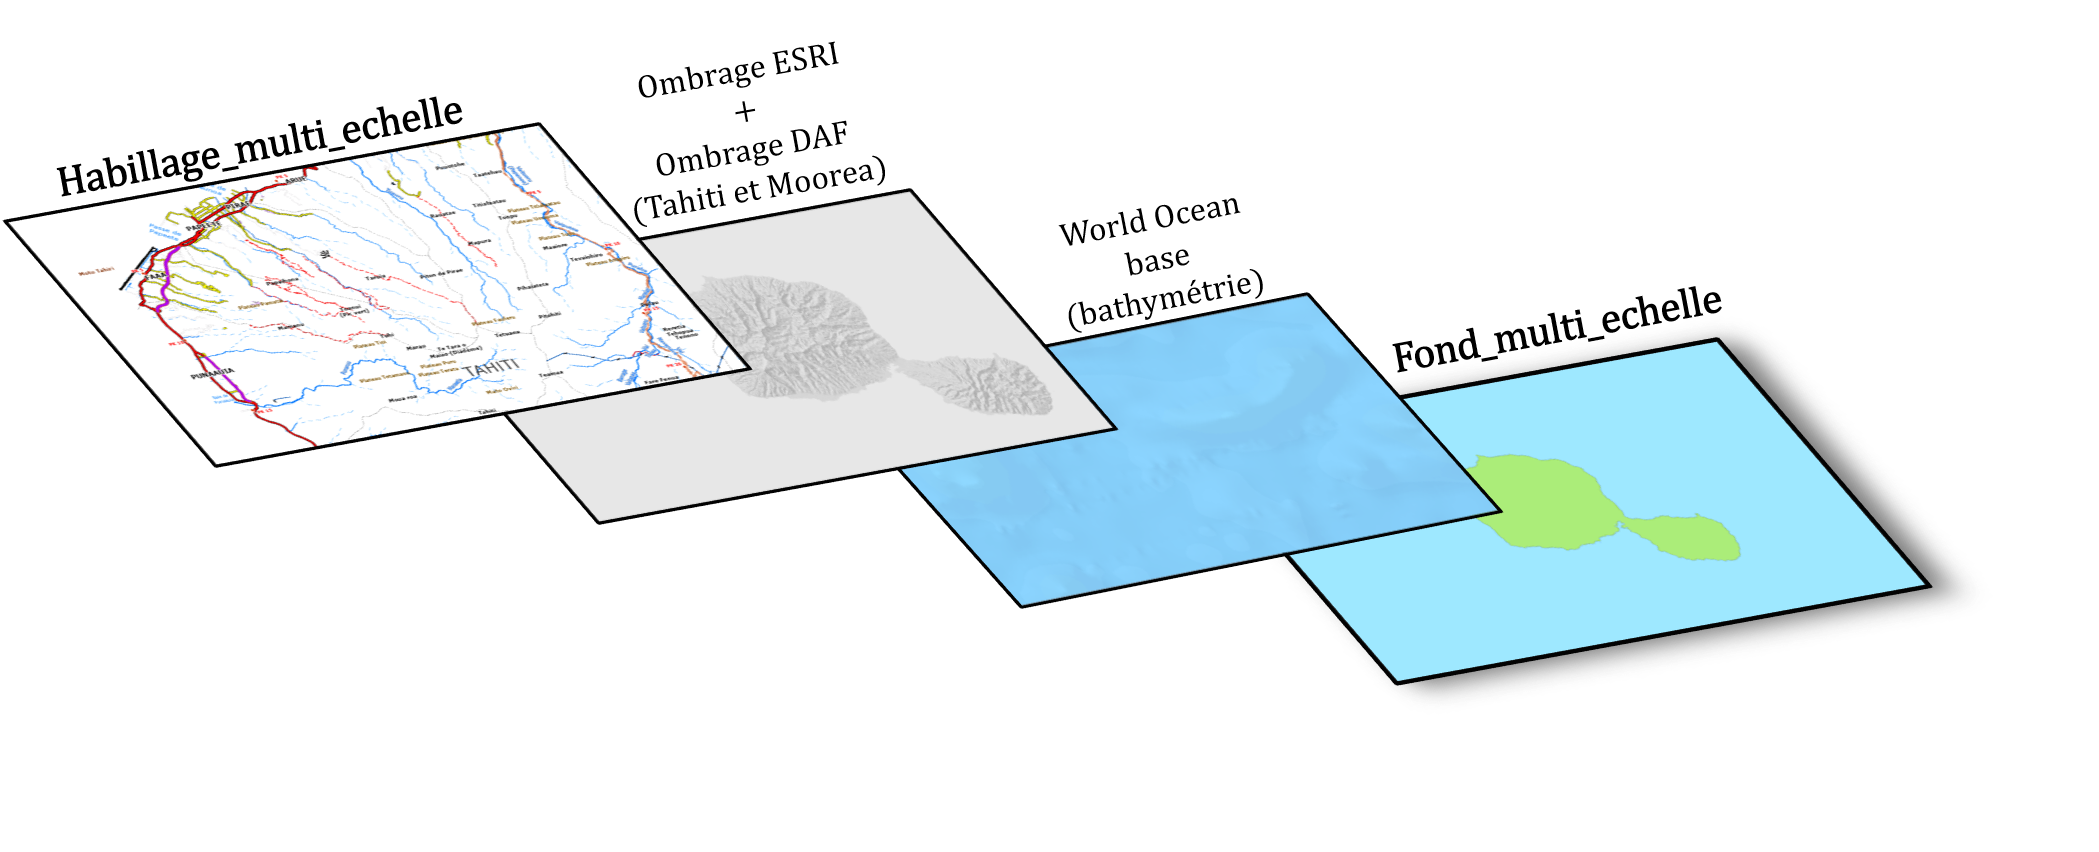
\includegraphics[width=\linewidth]{images/chap3/empilement.png}
\caption{Explication schématique de l'empilement des couches dans la carte web}
\label{empilement}
\end{figure}

Création d’un projet de fond de carte, contrainte de superposition: 

Chaque niveau de zoom comporte des couches situées au dessus de l’ombrage et d’autres en dessous (comme cela a été évoqué dans le chapitre précédente). La solution adoptée est donc une scission de la carte générale multi-échelle précédentes en deux cartes, l’une nommée Habillage\_multi\_echelle comportant pour chaque échelle, uniquement les couches destinées à être au dessus de l’ombrage et l’autre nommée Fond\_multi\_echelle comprenant uniquement des couches sur lesquels l’ombrage vient se superposer. Ces deux cartes ne comportent pas de données raster et sont exportées sur ArcGIS Online en tant que couches web du même nom. 

En ce qui concerne l’ombrage, ce dernier doit donc être placé entre les deux couches web précé- dentes. En utilisant la couche Terrain d’Esri, il est possible de ne pas avoir à exporter de données raster coûteuses sur ArcGIS Online. Mais comme en témoigne la figure 1.1 du chapitre 1, l’ombrage d’Esri est imprécis sur les zones montagneuses (souvent couvertes de nuages) de Tahiti. Il est donc utilisé à de petites échelles ne nécessitant pas un besoin important de précision et est combiné à un ombrage précis exporté sur une zone restreinte (Tahiti et Moorea) et pour des gammes d’échelles limitées dans l’optique de ne pas utiliser trop de crédits. Cette couche web nommée Ombrage\_TAH\_MOO est provisoire et doit être étendue sur toutes les îles hautes de la Polynésie française pour un rendu optimal sur le portail final. 



\section{Valorisation du fond de plan au travail d'applications thématiques}

\subsection{Géoportail et site web de la section topo}
{\color{magenta} Présenter les produits créés, comment les utiliser et leur vocation future (développement des thématiques en fonction des besoins)}

\subsection{Portail des fiches géodésiques et de nivellement}


 Qu'il s'agisse de cartes thématiques ( touristiques, de randonnée, etc...), de nombreux éléments peuvent être ajoutés à la carte actuelle. Par ailleurs, selon le thème choisi, il est possible de modifier l'habillage pour l'alléger et ainsi mettre en évidence cette thématique.

La dernière partie de ce projet qui concerne la diffusion des fiches géodésiques et de nivellement. L'objectif est de réaliser une version du portail qui soit spécialement consacrée à la diffusion de ces fiches pour les géomètres sur le terrain.
Il s'agit sur le portail précédemment créé, d'ajouter une couches des points de repère et de proposer au clic, une fenêtre contextuelle avec quelques information essentielles de la fiche ainsi qu'une photo. Le travail se découpe en plusieurs parties : 
\begin{itemize}
    \item Export depuis ARCGIS pro de la bonne version de la couche des repères avec la table des mesures associée
    \item Création sur Arcgis Pro d'une vue avec les éléments à diffuser
    \item Configuration de la fenêtre contextuelle avec les illustrations et les informations
    \item Ajout de la carte thématique au portail en ligne
\end{itemize}

{\color{magenta} Détailler les 4 items avec figures illustratives - ici, un bout seulement}

La fenêtre contextuelle doit contenir un condensé des éléments essentiels au géomètre qui devra trouver la majorité des renseignements nécessaires à cette endroit et pourra le cas échéant, accéder à la fiche pdf pour trouver des informations complémentaires. L'export qui à été décrit dans la partie ... permettait d'associer à la couche de donnée des pièces jointes incluant la photo au format jpeg ainsi que la fiche au format pdf. La fenêtre contextuelle doit d'abord faire figurer cette photo. Pour cela, un champ URL\_image doit être créé dans les champs de la couche pour y insérer le lien vers l'image en question. C'est par ce biais que l'image pourra être afficher dans la fenêtre contextuelle. La démarche de création du champ suit l'article de Gaetan Lavenu sur Arcorama \cite{lavenu} 

Cependant, la création du champ URL\_image différe de celui qui est proposé dans l'article car la couche des repères possède plusieurs pièces jointes et seules celles au format "image/jpeg" sont affichées dans la fenêtre. Le code permet donc de récupérer les id des pièces jointes désirées en les triant sur leur format selon qu'il s'agit de fiche pdf ou d'images jpeg. Ce code est expliqué en Annexe D. 
{\color{magenta} Détailler l'explication dans l'annexe}
\textsc{Remarques:} Une fois validée, la mise à jour du champ sur ArcGIS Online est particulièrement longue en ligne et nécessite environ 15 minutes pour 4000 éléments.


\section{Limites d'utilisation du portail}

\subsection {Limitations}
{\color{magenta} Détailler les problèmes  comme 
- les récifs
- les étiquettes
- l'absence de légende ( à voir avec ce qui a été déjà dit avant )
l'étiquetage sur les archipels et les cartes à des échelles supérieurs au 1/500 000. N'a pas été le principal thème de travail et les informations sont suffisantes sans être assez fournies avec quelques défauts d'étiquetage.
- l'ombrage imprécis d'esri+ Difficultés liées à la maintenance du portail et à la mise à jour des données}

\subsection {Axes d'amélioration}
Après avoir énuméré les limitations, cette sous-partie propose des axes d'amélioration pour la diffusion et la mise à jour d'un tel portail. 
{\color{magenta} 

- ombrage : soit la daf donne ses ombrages à esri pour éviter l'export assez coûteux (comme c'est le cas d'autres pays voir tableau). Ou alors export des ombrages. Problème, le nombre important d'îles hautes et donc d'ombrage. Le coût en crédit
- l'ombrage + Difficultés liées à la maintenance du portail et à la mise à jour des données}